\documentclass[a4paper,11pt]{article}
\usepackage[utf8]{inputenc}
\usepackage{titling}
\usepackage{url}
\usepackage{pbox}
\usepackage[margin=1in]{geometry}

\usepackage{graphicx}
\usepackage{hyperref}

\graphicspath{ {images/} }

\newcommand{\subtitle}[1]{%
	\posttitle{%
		\par\end{center}
	\begin{center}\large#1\end{center}
	\vskip0.5em}%
}

\title{Atlanta Pollen Counts Prediction}
\subtitle{BMED6700 Biostatistics, Final Project Report}
\author{Tomáš Brůna\thanks{Tomáš Brůna, 54675, bruna.tomas@gatech.edu},  
Dongjo Ban\thanks{Dongjo Ban, 42323, dban8@gatech.edu}, 
Saurabh Gulati\thanks{Saurabh Gulati, 24499, saurabhg59@gatech.edu}}

\begin{document}

\maketitle

\section*{Abstract}

Allergy is an incurable condition caused by the hypersensitivity of the immune system to something in the environment. Pollen, which is produced by flowering plants is one of the most common known allergen which causes symptoms as severe as impairment of cognitive performance. Pollen counts are expected to be correlated with weather, we thus attempted to predict future pollen levels based on historical pollen counts and weather data using time series models and machine learning algorithms. We are able to predict exact future pollen counts with mean absolute error of $\sim$3.4 and future pollen levels with $\sim$90\% accuracy.


\section{Introduction}
Allergies are among the most common chronic conditions affecting the global population. The symptoms range from minor inconveniences to life threatening reactions. Among the most common allergens that is known to trigger allergic responses is pollen \cite{kiotseridis2013grass}. Formed from flowering plants, airborne pollen may contain allergens that cause allergic inflammatory response which then could lead to a systemic reaction. Effect of the allergen includes not only nasal and ocular symptoms, but can also impair cognitive performance as well as information processing \cite{church2018allergic,bensnes2016you}.\\\\
Furthermore, as there is no cure for such allergies, it is of importance that people who are allergic make necessary adjustments to avoid contact with pollen. This makes predicting pollen levels an important activity to aid allergic individuals in taking the necessary steps required to stay well. Our project is focusing on such prediction based on historical pollen counts and weather data.
\section{Data Sources}

\subsection{Pollen Counts Data}
Pollen data was sourced form the Atlanta Allergy portal - \url{www.atlantaallergy.com}. This website contains Atlanta's polled count for almost every day from June 1991 up to today. For any particular day they have the total pollen count and also the individual pollen categories for tree, weed and grass pollen. The categories are either \textit{Extreme (E)}, \textit{High (H)}, \textit{Medium (M)} or \textit{Low (L)}. For some days they also have the top contributor for the different pollen categories. The data resides on the website in the form of a calender showing the above mentioned information, hence we decided to write a web-scraping script to extract the information.
\subsubsection{Scraping}
Data for each day reside at a unique URL. For example, pollen counts for May 14, 2002 are located at \url{http://www.atlantaallergy.com/pollen_counts/index/2002/05/14}. We designed a script which iterates through each day and corresponding URL since June 18, 1991 (first entry) up to today. Next step was to extract pollen counts and pollen levels for different categories from these pages. Several special cases such as days with missing or invalid values needed to be handled. The scripts saves all the results into a single tab separated file with the following columns: \emph{Year, Month, Day, Total Count, Tree Level, Tree Top Contributors, Grass Level, Grass Top Contributors, Weed Level, Weed Top Contributors}. We attached the full script in the \texttt{scraper.py} file. To test, just run \texttt{./scraper.py} and the result will be saved in \texttt{out.tsv} file.

\subsection{Weather Data}

The weather data was sourced from Weather Underground (\url{https://www.wunderground.com/}). Weather underground is a weather service that provides accurate real-time weather information; the information in Weather Underground comes from the National Weather Service and from 250,000 Personal Weather Stations, making it the most reliable source of weather data available. The National Weather Service, which is part of the National Oceanic and Atmospheric Administration (NOAA), and is considered the standard for most climate and weather data related research. We collected location specific information of weather in Atlanta and matched the time range to the available pollen data. 
\subsubsection{Scraping}
We extracted historical weather information, ranging from 1991 until present day, using Beautiful Soap, a python package for parsing HTML and XML documents. In order to stay consistent with the pollen counts dataset, we set the location to Atlanta, Georgia. Using the scraper, we parsed through the monthly weather data that consisted of temperature, wind speed, precipitation, humidity, and weather events.

\section{Dataset Description}
\subsection{Merging Datasets}
Once the weather and pollen data were scraped from the individual sources, we merged the datasets based on the date. By merging we got a dataset which had both the pollen and weather information for most days starting June 1991 till today.\\\\
The merged dataset has all of the described pollen data and weather information: \textit{Temperature, Humidity, Precipitation, Wind Speed, Dew Point, Sea Level and the Weather Events} that occurred on that day. Since the websites were missing the data for some days, the merged dataset had some of the data missing. For more details, see the included \texttt{mergedData.csv} file.
%\subsection{Format Description}
\subsection{Handling Missing Values}
To handle missing values in the merged dataset, we used R package \textit{imputeTS} \cite{moritz2015imputets} which is a collection of algorithms and tools for univariate time series imputation. Linear interpolation was used to impolate the missing values for Weather columns and total pollen counts. Once the data was interpolated, it was ready for the time series analysis.

\section{Time Series Analysis}

Time series consists of sequential numerical data in successive order. Its application range from social setting, such as economics and unemployment, to areas of health where an effect of a certain drug type is measured over time. One of the most rigorous and advanced practice involves environmental sciences.\\\\
The pollen data we extracted consists of discrete time data measuring daily pollen counts. In order to derive meaningful statistics and to analyze the dataset, we chose to perform time series analysis. With this method, we will be able to achieve our primary goal of being able to predict the number of pollen counts for a given day of a year by utilizing the seasonal and past data \cite{timeseries1}.

\subsection{Exploratory Analysis}

Visualizing the time series plots before performing any statistical tests can give an insight as to how to move forward with the analysis. It is considered to be one of the important topics in environmental analysis as it can assist in identifying and understanding association between the data. The visualization is displayed in the Figure \ref{fig:exploratory1}.\\

\begin{figure}
	\centering
	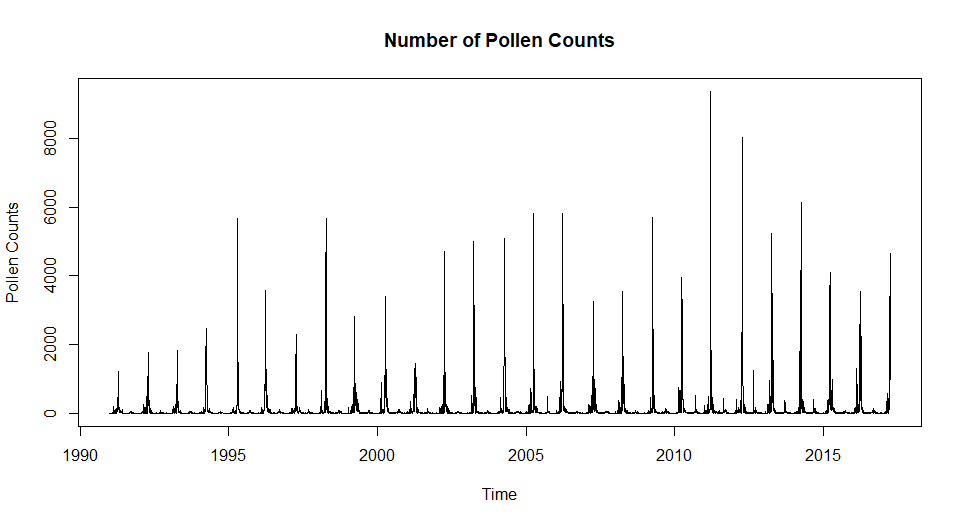
\includegraphics[width=0.9\textwidth]{Exploratory1}
	\caption{Number of pollen counts from 1991 to 2018.}
	\label{fig:exploratory1}
\end{figure}

\noindent
Initial screening of the pollen counts throughout the years does not offer a definite answer as to whether our dataset contains a trend or not. It does, however, show that the counts reached its peak around 2011. A quick search was done to inspect a possible cause for sudden rise of pollen level, but there were no significant findings. In order to examine our time series more in depth, we decomposed our time series into 3 different components: seasonal, trend, and residuals (Figure \ref{fig:ExploratoryDecomp}).\\

\begin{figure}
	\centering
	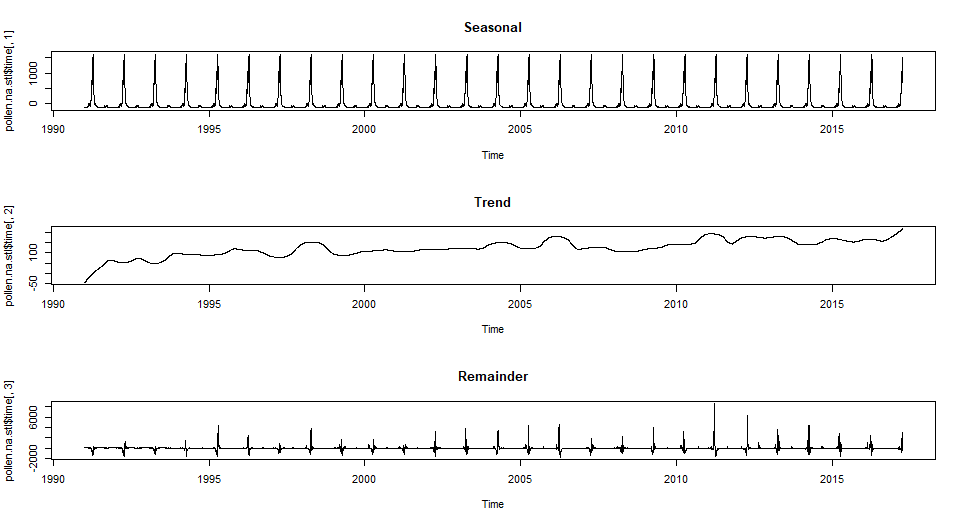
\includegraphics[width=0.9\textwidth]{ExploratoryDecomp}
	\caption{Decomposition of pollen count time series data.}
	\label{fig:ExploratoryDecomp}
\end{figure}

\noindent
After the decomposition, we can observe that seasonality is consistent throughout the years with peaks happening around the same time period. We can also notice consistency in residuals, with largest peak occurring around the same time where our time series was at its highest. The trend seems to be the only component from decomposition that is not consistent and showing a deterministic trend as year progresses.

\subsection{Tests for Stationarity}

Stationarity is essential in research where the variables are dependent on time. Thus, it is an important assumption that precedes making any type of predictions or forecasts. In order to determine whether our pollen count data is stationary or not, we employed two statistical tests: augmented Dickey-Fuller and KPSS \cite{keblowski2004adf}.\\\\
Unit root tests are generally used to determine if the trending data needs to be differenced or regressed on some function of time to make it stationary \cite{diebold2000unit}. Developed by Said and Dickey in 1984, augmented Dickey-Fuller expands the autoregressive unit root test to handle ARMA models, allowing it to handle more complicated autoregressive model.
$$H_0:\ time\  series\  is\  nonstationary$$
$$H_1:\ time\ series\ is\ stationary$$
We carried out the statistical test using `tseries' R package and observed a p-value smaller than 0.01. Therefore, we reject the null in this case and can say that our time series is stationary and does not require detrending. It is a common practice to perform more than one test to determine stationarity of the time series of interest. More specifically, Kwiatkowski–Phillips–Schmidt–Shin (KPSS) test is jointly used with augmented Dickey-Fuller test (ADF). 
$$H_0:\ time\ series\ is\ stationary$$
$$H_1:\ time\  series\  is\  nonstationary$$
We can notice that the hypotheses are different from ADF. Using the same package as ADF, we performed another statistical test and observed a p-value greater 0.1. Thus, we cannot reject the null hypothesis and can say that our time series is stationary. 

\subsection{Model Fitting}
The aim of fitting a model for a time series is to be able to incorporate past observations from the series to create a model that best describes the characteristics of the series \cite{DBLP:journals/corr/abs-1302-6613}. One of the most popular and widely used time series model is autoregressive moving average (ARMA) model.
Using auto.arima() function in `forecast' package in R, we are able to predict best parameters for ARMA model using AIC or BIC scores. The resulting model for our pollen counts data was ARMA(3,2) \cite{hyndman2007automatic}.\\

\begin{figure}
	\centering
	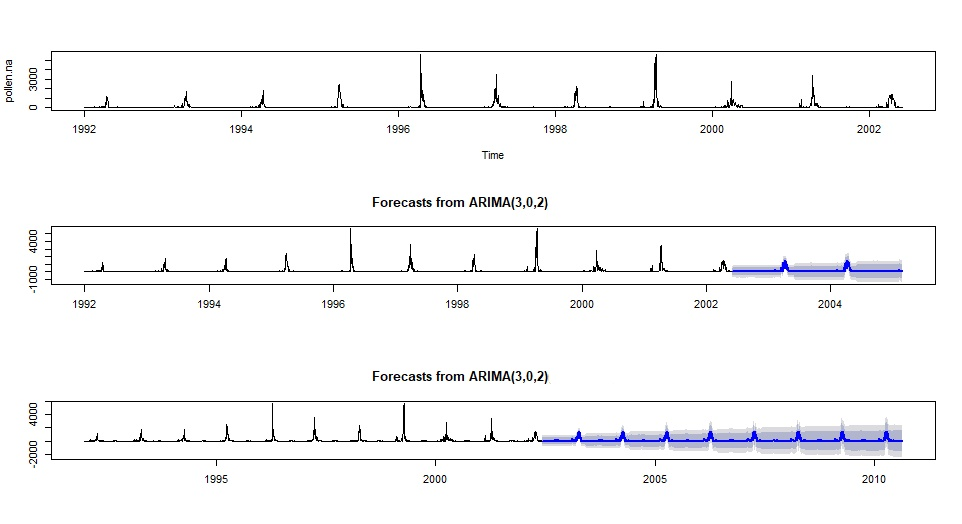
\includegraphics[width=0.9\textwidth]{InkedPredict3_LI.jpg}
	\caption{Top: original data; Middle, Bottom: Forecasts based on the predicted ARMA model.}
	\label{fig:ExploratoryACF}
\end{figure}
\noindent
Using the fitted model, we performed two predictions: 2 years and 8 years into the future. From the predictions, we notice that they depend on the shape and height of the peak near the end. Furthermore, we see the confidence interval for both predictions increasing. See Figure \ref{fig:ExploratoryACF} for details. This increase is reasonable considering the level of error and uncertainty would increase as time progresses.
\subsection{Time Series Conclusion}

From the exploratory analysis, we noticed a seasonal pattern where pollen counts experience a dramatic increase. Moreover, we became aware of the trend in our dataset. However, we learned that our pollen counts dataset is stationary and does not require any type of detrending by performing statistical tests for stationarity. Furthermore, the predictions seem to be relatively close to the overlapping original data. They also seems to stay constant for the most part, mimicking the peak at the end of the plot. Lastly, we can also notice confidence interval slowly increasing.\\\\Examining the ACF plot (Figure \ref{fig:ExploratoryACF2}) shows us that pollen counts for the current day depends not only on the past couple of days or weeks, but also on the same day of previous years as well.

\begin{figure}
	\centering
	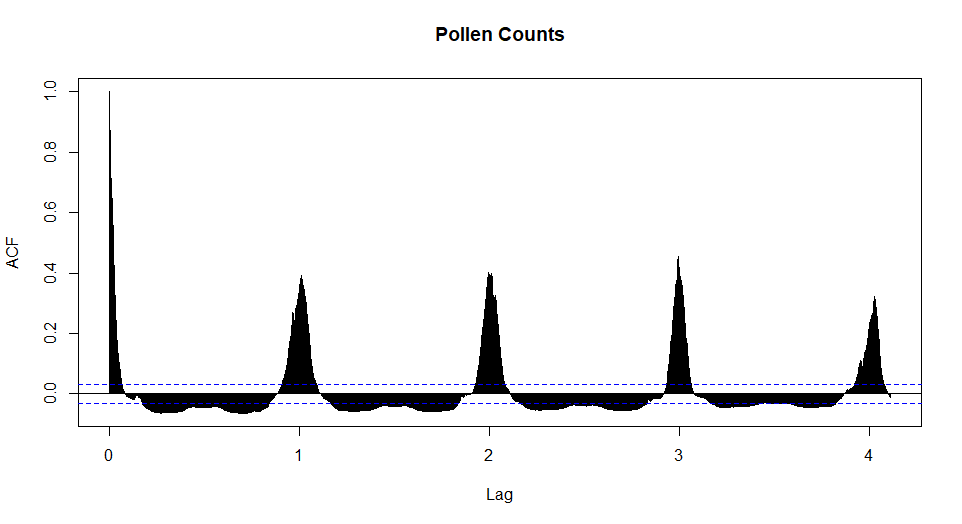
\includegraphics[width=0.9\textwidth]{PollenACF1000.png}
	\caption{ACF plot with lag 4}
	\label{fig:ExploratoryACF2}
\end{figure}

\section{Machine Learning}

Apart from using seasonal and past pollen data, we decided to add more explanatory variables to help us predict the future pollen counts. We chose weather data for this purpose because pollen counts are expected to be highly correlated to weather. For example, rain can wash the pollen away and water associated with increased humidity weighs the pollen grains down so they do not travel as far when the wind blows.\\\\
Weather data have the advantage of being closely and precisely monitored. Apart from that, reliable weather forecasts are usually available, therefore we can base our future predictions on the weather forecasts.\\\\
Due to the high number of explanatory weather variables which can interact with each other and affect pollen counts in a nonlinear fashion, we decided to use supervised machine learning algorithms. We tested neural networks and random forests which are designed to handle such interactions as well as other methods such as linear regression. In general, supervised machine learning maps input data (weather, season and past pollen counts) to output which are future pollen counts.

\subsection{Weather Data Only}
To see how well the weather explains pollen counts (without using the past pollen data), we based our first set of models on the day of the year (representing seasonality) and the weather data only. This approach assumes the availability of a reliable weather forecast on which the prediction for the future pollen counts will be based\footnote{This is not an issue when prediction few days into the future (which is what we are trying to do). However, long term predictions using this approach are not possible due to the limitations of weather forecasts.}.\\\\
This method has several advantages: Since it does not use any past information, the rows are independent and any rows with missing values can be ignored during the model training. Also, predictions can be made even when past pollen counts are not available.

\subsubsection*{Algorithms}
We compared four different regressors:
\begin{itemize}
	\item Linear regression \cite{seber2012linear}
	\item Neural network \cite{haykin2004comprehensive}
	\item Support Vector Machine \cite{suykens1999least}
	\item Random Forest \cite{liaw2002classification}
\end{itemize}
\subsubsection*{Parameter Estimation} For a fair comparison, we tried to find a set of optimal parameters for the methods. This was achieved by running each of the algorithms multiple times with changing parameters and measuring the proportion of variance explained ($R^2$) \cite{carpenter1960principles}. To account for overfitting and estimate the true performance of each model, we measured $R^2$ using 10-fold cross-validation \cite{kohavi1995study}.
See Table~\ref{tab:optimal} in the Appendix for a list of optimal parameters found for each algorithm.
\subsubsection*{Results}
The final $R^2$ scores for each of the methods are displayed in the Table \ref{tab:regressors}. The table shows that the performances of Neural network, Support vector machine and Random forest are comparable.\\
\begin{table}
	\centering
	\begin{tabular}{cllll}
		\hline \\
		\vspace{0.6em}
		Algorithm & \pbox{20cm}{Linear \\ Regression} & \pbox{20cm}{Neural \\ Network} & \pbox{20cm}{Support Vector \\ Machine}  &\pbox{20cm}{Random \\ Forest}  \\
		\hline \\
		\vspace{0.2em}
		$R^2$ & 0.002 & 0.34  & 0.334 & 0.346 \\ \vspace{-0.4em} \\
		\hline
	\end{tabular}
	\caption{A comparison of $R^2$ scores for different regressors. Weather and seasonal data are used to predict pollen counts. The higher the score, the better the model is. All models were run with a set of best parameters found.}
	\label{tab:regressors}
\end{table}

\noindent
Neural networks are extremely sensitive to parameter setting. We observed that a small change in the number of neurons can bring the $R^2$ performance to almost 0. Support vector machines are more robust to parameter changes, however, the explanatory features need to be normalized prior to model training and the training itself takes a relatively long time. The Random forest is robust with respect to parameter settings and the training time is almost instant compared to SVM. Therefore, Random forest is the model we recommend for pollen count predictions and we will focus on random forests in the following analyses. Table \ref{tab:scores} shows additional qualitative measures for the Random forest.
\begin{table}
	\centering
	\begin{tabular}{lr}
		\hline \\
		\vspace{0.6em}
		Measure & \pbox{20cm}{Random \\ Forest}  \\
		\hline \\
		\vspace{0.2em}
		$R^2$ & 0.346 \\ 
		\vspace{0.2em}
		Mean Absolute Error & 99.817 \\
		\vspace{0.2em}
		Median Absolute Error & 5.316 \\ \vspace{-0.4em} \\
		\hline
	\end{tabular}
	\caption{Error measures for Random forest regressor. Weather and seasonal data are used to predict pollen counts.}
	\label{tab:scores}
\end{table}

\subsection{Inclusion of Historical Pollen Counts}
\label{sec:history}
The time series analysis showed us that pollen counts are highly correlated to pollen count levels from the past several days (see Figure \ref{fig:ExploratoryACF}). Therefore, it makes sense to include this information to achieve better predictions -- we added values of pollen counts for the past 8 days among our explanatory variables. Because of that, each row depends on the 8 previous rows -- dropping a row with missing values would also affect the subsequent 8 rows. Thus, we needed to impute the missing values in this case. Again, we used Random forest regressor as our model and cross-validation to evaluate the performance.

\subsubsection*{Results}
Inclusion of the recent pollen counts significantly improved the performance of our model. Table \ref{tab:future} summarizes the prediction errors. Analysis of decision trees in the fitted Random forest model shows (not surprisingly) that the most important splitting attribute is the value of pollen counts in the $day - 1$. The weather and seasonality are still used in the lower levels of the tree.

\begin{table}
	\centering
	\begin{tabular}{crrrrr}
		\hline \\
		\vspace{0.6em}
		Future prediction & 1 day & 2 days & 3 days  & 4 days & 5 days  \\
		\hline \\
		\vspace{0.2em}
		$R^2$ & 0.755 & 0.617 & 0.49  & 0.422 & 0.429 \\ 
		\vspace{0.2em}
		Mean Absolute Error & 56.244 & 75.296 & 85.911  & 95.218 & 97.924\\
		\vspace{0.2em}
		Median Absolute Error & 3.395  & 5.157 & 6.391  & 7.119& 7.998  \\ \vspace{-0.4em} \\
		\hline
	\end{tabular}
	\caption{Performance of Random forest predictions (with weather, seasonal and recent pollen counts explanatory data) with respect to how many days in the future we are predicting.}
	\label{tab:future}
\end{table}

\noindent
This type of prediction can only predict pollen counts one day into the future (because it needs data from $day-1$). We also show how the prediction accuracy changes when we predict more than one day into the future. This is achieved by deleting column $day-1$ when prediction 2 days into the future, deleting $day-1$ and $day-2$ when prediction 3 days etc. The behavior of accuracy with increasing future days is shown in the Table \ref{tab:future}.

\begin{table}
	\centering
	\begin{tabular}{crrrrr}
		\hline \\
		\vspace{0.6em}
		Future prediction & 1 day & 2 days & 3 days  & 4 days & 5 days  \\
		\hline \\
		\vspace{0.2em}
		$R^2$ & 0.732 & 0.597 & 0.484  & 0.419 & 0.387 \\ 
		\vspace{0.2em}
		Mean Absolute Error & 59.352 & 79.090 & 89.529  & 98.030 & 101.293\\
		\vspace{0.2em}
		Median Absolute Error & 3.345  & 5.120 & 6.156  & 7.291& 7.747  \\ \vspace{-0.4em} \\
		\hline
	\end{tabular}
	\caption{Performance of Random forest predictions (with seasonal and recent pollen counts explanatory data) with respect to how many days in the future we are predicting.  Compared to table \ref{tab:future}, this model is not using weather data at all.}
	\label{tab:futurenoweather}
\end{table}


\subsubsection*{Removing Weather}

We also measured the performance of this model without any weather data. The result is displayed in the Table \ref{tab:futurenoweather}. This result shows that recent and seasonal pollen data are more important explanatory variables than weather. The importance of weather increases the more days in the future we are trying to predict. 

\subsection{Machine Learning Conclusion}

Overall, we recommend to use both weather and historical pollen data for model fitting and predictions. Even though the historical pollen counts are better explanatory variables, weather still improves the predictions and might be crucial when the observations for past pollen count levels are not available.

\subsection{Pollen Category Level Prediction}
So far in our analysis, we focused on predicting the total pollen counts. Apart from overall counts, the data from \url{http://www.atlantaallergy.com/} also contain pollen levels for three categories: \emph{tree}, \emph{weed} and \emph{grass}. Predicting these individual categories can be important since people can be sensitive only to some of these pollen types.\\\\
The values for these categories are not continuous, there are only 4 possible labels: \textit{Extreme (E)}, \textit{High (H)}, \textit{Medium (M)} or \textit{Low (L)}. Therefore, predicting these labels becomes a classification instead of a regression problem.

\subsubsection*{Method and Results}
Using the knowledge and observations from the previously described experiments, we use the following method to predict pollen levels in distinct categories: First, we use only weather and seasonal data to train a Random Forest model. Because linear imputation of missing values is not a robust option for filling in missing categorical values \cite{allison2005imputation}, we use this model to predict pollen level for rows with missing values.\\\\
Next step is to include data from past 8 days (described in Subsection \ref{sec:history}) and measure the prediction accuracy. The result is summarized in Table \ref{tab:category}. The tables show that prediction of pollen levels can be done very accurately ($\sim$90\% accuracy) with Random forest classifier for each of the pollen categories. It is also worth noting that the prediction quality remains high even when pollen data from past 5 days are not available. 


\begin{table}
	\centering
	\begin{tabular}{lrr}
		\hline \\
		\vspace{0.6em}
		Explanatory Variable & \pbox{30cm}{Weather \\ \& Season} & \pbox{30cm}{Weather \\ \& Season \\ \& History}   \\
		\hline \\
		\vspace{0.2em}
		Accuracy for tree pollen levels & 0.820 & 0.872 \\ 
		\vspace{0.2em}
		Accuracy for weed pollen levels& 0.864 & 0.924 \\
		\vspace{0.2em}
	    Accuracy for grass pollen levels& 0.897  & 0.925  \\ \vspace{-0.4em} \\
		\hline
	\end{tabular}
	\caption{Prediction accuracies for pollen levels in each of the pollen categories. Random Forest classifier and cross-validation are used. In case of column where past data are used as explanatory variable, accuracy of 1 day future prediction is displayed.}
	\label{tab:category}
\end{table}


\section{Conclusion}
In this project, we successfully employed time series analysis and machine learning to predict future pollen numbers. Time series results show that we are able to predict the pollen counts to a certain extent, but the model is not able to capture accurately how our series is behaving. Concerning machine learning, we are able to predict pollen levels much more accurately than the exact pollen counts. This might be sufficient for real-world application because prediction of general pollen concentration for different pollen categories is more important from the medical standpoint than the precise overall pollen count number. This prediction will enable people who are allergic to the specific pollen type to take the necessary precautions. 

\subsection*{Lessons Learned}
In the first part of the course, we learned to apply several statistical tests on real biological data. The course was especially useful in showing us how these tests differ from each other and in which context they should be used.\\\\
Next part of the class was also very helpful because we covered essential biological methods: how to account for multiple comparisons and time series.\\\\
Last but not least, this project taught us key concepts related to time series and we also gained hands-on experience with using supervised machine learning for both classification and regression.
\bibliography{mybib}{}

\bibliographystyle{iso690}

\section*{Appendix}

\subsection*{Optimal Machine Learning Parameters}
\begin{table}[h!]
	\centering
	\begin{tabular}{llll}
		\hline \\
		\vspace{0.6em}
		Algorithm & Important Parameters &  &    \\
		\hline \\
		\vspace{0.2em}
		Neural Network & $hidden\ layers=2$ & $layer\ 1\ neurons=10$  & $layer\ 2\ neurons=10$ \\
		\vspace{0.2em}
		Support Vector Machine & $C=100$ & $Kernel=rbf$  &   \\
		\vspace{0.2em}
		Random Forest & $max\ tree\ depth=4$ & $num\ trees=25$  & $criterion=mse$  \\ \vspace{-0.4em} \\
		\hline
	\end{tabular}
	\caption{Optimal parameters found for different machine learning algorithms. Only the important parameters affecting performance the most are displayed. Weather and seasonal data were used to predict pollen counts.}
	\label{tab:optimal}
\end{table}



\end{document}
